
- [x] (1) Audience: lower-level visualization library developers, domain specific library developers (continuing the architecture choices mpl made)

- [x] (3) Proposed solution: 
    - [x] functional math model, structure/type preserving 
-  [x] (4) Novelty:
    - [x] functional architecture
    - [x] explicitly expressing continuity in the model
    - [x] model is constraint oriented rather than evaluative
- [x] (5) Benefits: 
    - [x] functional: robustness, concurrency, modularity, proves that reliably, backfit needs to this 

- [x] (2) Need: unified model: continuity + equivariance 
    - [x] mpl works, unmaintainable, grew organically, this stuff is buried implicitly, gives a way to make it clear
    - [x] interactivity screen space back to data space, different implicit data than API incoherancy than bug?
        - [x] currently done in adhoc manner, want to enforce contracts for the interactivity 
    - [x] redesign that reliably enforces these constraints 
    - [x] library that supports all the data 
        - [x] relational tables, and images, and data cubes (with coordinates), and networks, and other data structures
        - [x] streaming and concurrency 
        - x blob the same? - model explains why this should be true
    - [x] framework to enforce invariance at the architecture level
    - [x] match engineering w/ math

- [x] (6) Evaluation: The method of evaluation to verify that the proposed solution delivers the stated benefits must be given.
        The best justifications explicitly discuss particular choices in the context of several possible alternatives.
        1. Case studies in the form of implementations (is this feasible) 
        2. Comparison w/ existing implementation     

- [ ] (7) More specific discussion of what will be done and on what timeline.
        [quarterly gantt charts?]
[] close out board https://github.com/story645/proposal/projects/3



The work presented in this paper is motivated by a need for a library of visualization components that developers could use to build complex, domain specific tools tuned to the semantics and structure carried in domain specific data. While many researchers have identified and described important aspects of visualization, they have specialized in such different ways as to not provide a model general enough to natively support the full range of data and visualization types many general purpose modern visualization tools may need to support. The core architecture also needs to be robust to the big data needs of many visualization practitioners, and therefore support distributed and streaming data needs. To support both exploratory and confirmatory visualization\cite{tukeyWeNeedBoth1980}, this tool needs to support 2D and 3D, static, dynamic and interactive visualizations. 

Specifically, this work was driven by a rearchitecture of the Python visualization library Matplotlib\cite{hunterMatplotlib2DGraphics2007} to meet modern data visualization needs. We aim to take advantage of developments in software design, data structures, and visualization to improve the consistency, composibility, and discoverability of the API. To do so, this work first presents a mathematical description of how data is transformed into graphic representations, as shown in figure~\ref{fig:intro_artist_stages}. As with other mathematical formalisms of visualization \cite{mackinlayAutomatingDesignGraphical1986,kindlmann2014algebraic,sugibuchiFramwork2009,vickersUnderstandingViz2013}, a mathematical framework provides a way to formalize the properties and structure of the visualization. In contrast to the other formalisms, the model presented here is focused on the components that build a visualization rather than the visualization itself. 

In other words this model is not intended to be evaluative, it is intended to be a reference specification for visualization library API. To make this model as implementation independent as possible, we propose fairly general mathematical abstractions of the data container such that we do not need to assume the data has any specific structure, such as a relational database. We reuse this structure for the graphic as that allows us to specifically discuss how structure is preserved. We take a functional approach because functional paradigms encourage writing APIs that are flexible, concise and predictable due to the lack of side effects \cite{loudenProgrammingLanguagesPrinciples2010}. Furthermore, by structuring the API in terms of composition of the smallest units of transformation for which we can define correctness, a functional paradigm naturally leads to a library of highly modular components that are composable in such a way that by definition the composition is also correct. This allows us to ensure that domain specific visualizations built on top of these components are also correct without needing knowledge of the domain. As with the other mathematical formalisms of visualization, we factor out the rendering into a separate stage; but, our framework describes how these rendering instructions are generated. 

In this work, we present a framework for understanding visualization as equivariant maps between topological spaces. Using this mathematical formalism, we can interpret and extend prior work and also develop new tools. We validate our model by using it to re-design artist and data access layer of Matplotlib, a general purpose visualization tool.

\subsection{Visualization}

\begin{figure}[H]
    \begin{subfigure}{.24\textwidth}
        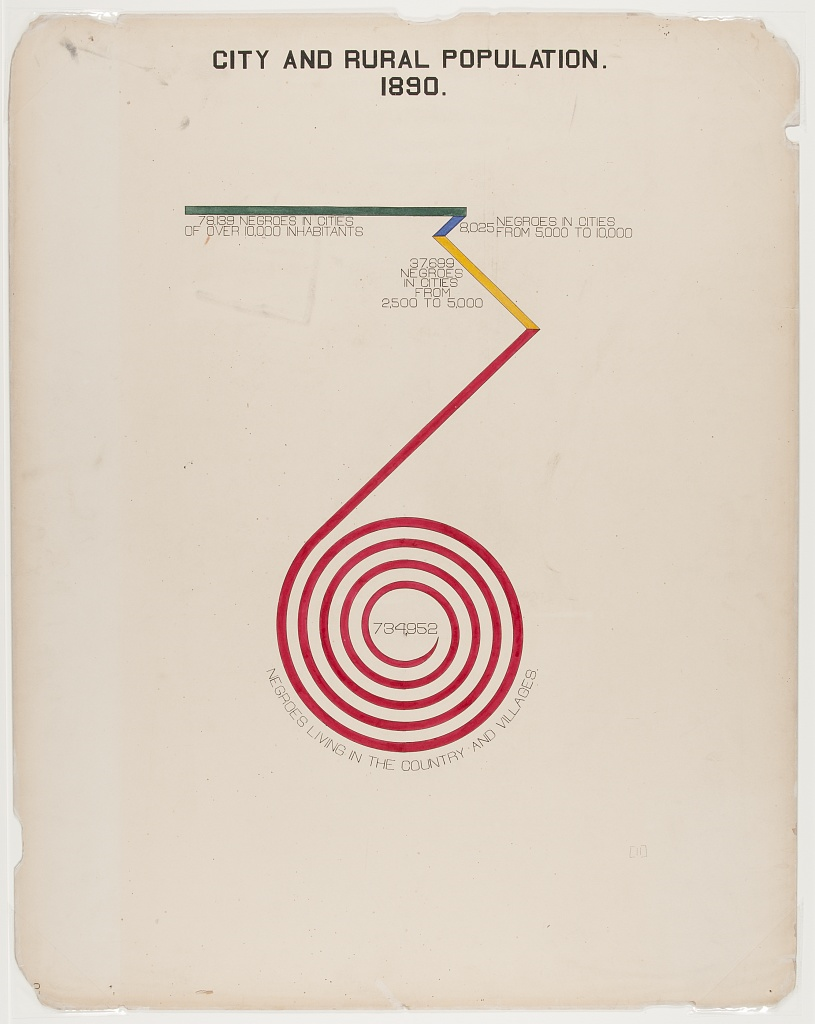
\includegraphics[width=1\textwidth]{figures/intro/du_bois_spinny.png}
        \caption{}
        \label{fig:intro_dpa}
    \end{subfigure}
    \begin{subfigure}{.24\textwidth}
        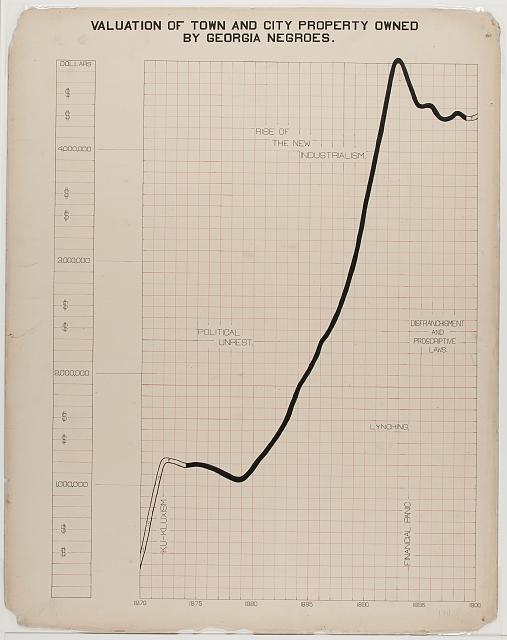
\includegraphics[width=1\textwidth]{figures/intro/du_bois_line.png}
        \caption{}
        \label{fig:intro_dpb}
    \end{subfigure}
    \begin{subfigure}{.24\textwidth}
        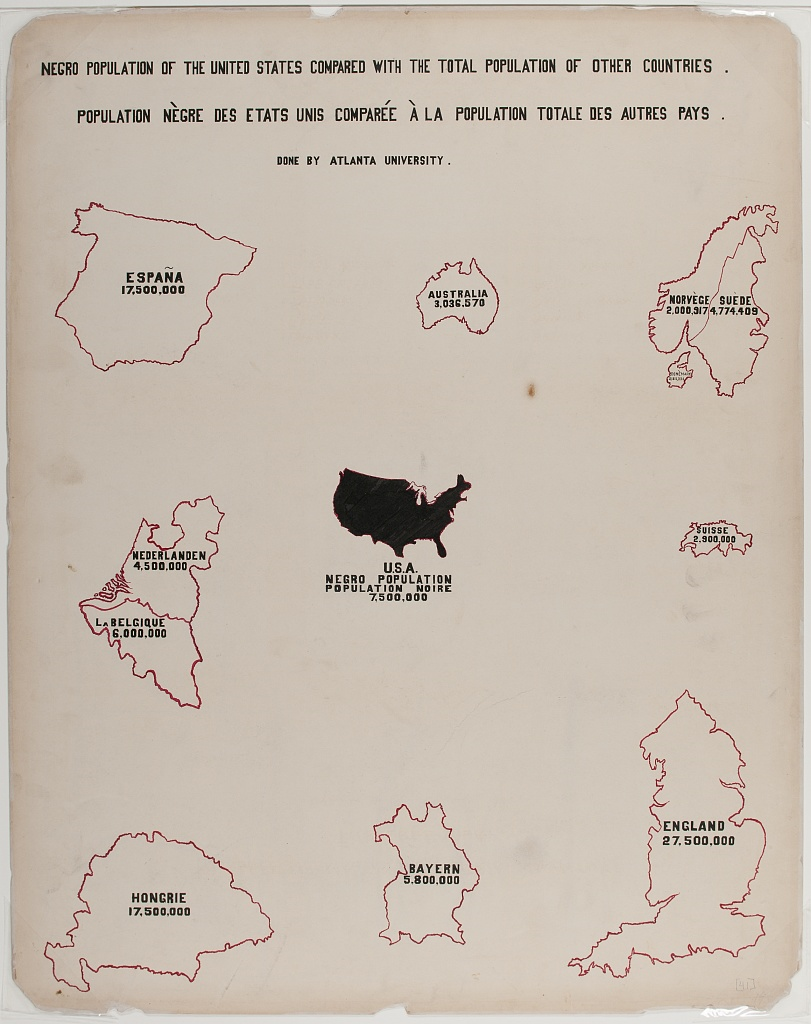
\includegraphics[width=1\textwidth]{figures/intro/du_bois_country.png}
        \caption{}
        \label{fig:intro_dbc}
    \end{subfigure}
    \begin{subfigure}{.24\textwidth}
        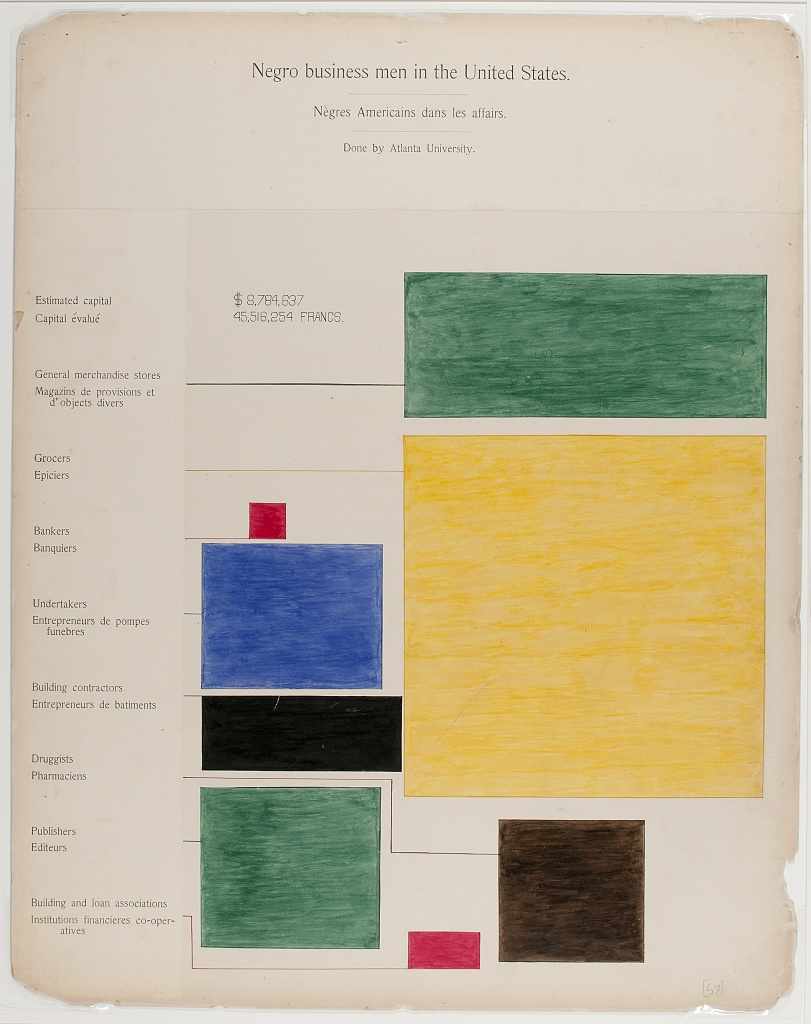
\includegraphics[width=1\textwidth]{figures/intro/du_bois_heat.png}
        \caption{}
        \label{fig:intro_dbd}
    \end{subfigure}
    \caption{Du Bois' data portraits\cite{duboiscenterattheuniversityofmassachusettsBoisDataPortraits2018} of post reconstruction Black American life exemplify that the fundemental characteristics of data visualization is that the visual elements vary in proportion to the source data. In figure~\ref{fig:intro_dpa}, the length of each segment maps to population; in figure~\ref{fig:intro_dpb}, the line changes color to indicate a shift in the political environment; in figure~\ref{fig:intro_dbc} the countries are scaled to population size; and figure~\ref{fig:intro_dbd} is a treemap where the area of the rectangle is representative of the number of businesses in each field. The images here are from the Prints and Photographs collection of the Library of Congress \cite{duboisGeorgiaNegroCity1900,duboisGeorgiaNegroValuation1900, duboisSeriesStatisticalCharts, duboisSeriesStatisticalChartsa}}
    \label{fig:intro_dubois}
\end{figure}

One example of highly expressive visualizations are the data portraits by Du Bois shown in figure~\ref{fig:intro_dubois}. While the Du Bois charts are different from the usual scatter, line, and plot charts, they conform to the constraint that a graphic is a structure preserving map from data to visual representation. Figure~\ref{fig:intro_dpa} is semantically similar to a bar chart in that the lengths of the segments are mapped to the values, but in this chart the segments are stacked together. Figure~\ref{fig:intro_dpb} is a multicolored line chart where the color shifts are at periods of political significance. In figure~\ref{fig:intro_dbc}, Du Bois combines a graphical representation where glyph size varies by population with a figurative representation of those glyphs as the countries the data is from, which means that the semantic and numerical properties of the data are preserved in the graph. Figure~\ref{fig:intro_dpd} is simply a treemap\cite{heerTourVisualizationZoo2010} with space between the marks. Since the Du Bois data portraits meet the criteria of a faithful visual representation, we propose a mathematical framework and implementation that allows us to express the Du Bois charts and common chart types with equal fidelity. 


Associativitly means (a*b)*c = a*(b*c), as you know. Replace * with whatever binary operator you like. Same thing. Key one for CS/cat theory is when a, b, c are functions and * is composition. When you have something that seems like it always holds (like associativity does for function composition and most operations you can think of), it can be confusing because it is like .... why do you need to check this? it always has to be true.
It turns out that it isn't for some binary operators that can be useful but we just don't see unless we are making general statements.
But when you are proving something, it is important step in the proof.
Part of the fact that the composition of equivariant functions eg. \nu and Q is equivariant, relies on the associativity. It just seems so obvious that you don't notice it, but if things wheren't associative .... suddenly all kinds of equations you are writing down and moving parenthesis, would either NOT be true, or be much more complicated.
one way to write equivariance (for a group at least) as invariance is
g^-1*\nu(g*\tau) = \nu(\tau)
just imagine if order of operations between function call and g* mattered... it is hard because function composition IS associative but if it wasn't you couldn't just write that.
There is an algebra called the octonians which is NOT associative but has a more complicated function so you can relate a*(b*c) with (a*b)*c with a isomorphic map (just isn't equal). Every equation becomes a mess. So the bottom line is that in a definition or a proof you might have to whip out associativity, but most of the time it does "just hold". It is mentioned when needed, but it isn't a serious constrain like continutity or equivariance ... it mostly "just holds".

monoid -> set w/ associativity and identity

set = R, f: R->R, 
composotion of functions from a space to itself, is associative (\compo)

S
This API choice can lead to visualizations that break \textit{continuity} when fed into visualizations with different assumptions about structure. The lack of consistent data model can also mean no consistent way of updating the data and therefore no way of guaranteeing that the views are in sync, in visualizations that consistent of multiple views of the same datasource, such as dashboards\cite{a.sarikayaWhatWeTalk2019,fewDashboardConfusionRevisited2007}. 